\documentclass[border=0pt]{standalone}
\usepackage[scaled]{helvet}
\renewcommand\familydefault{\sfdefault}
\usepackage{tikz}
\usetikzlibrary{arrows.meta, calc}

% ---------------- colours ----------------
\definecolor{blobYellow}{HTML}{FBE8A6}
\definecolor{blobBlue}{HTML}{B9DCF3}
\definecolor{blobRed}{HTML}{F6C2B6}
\definecolor{blobGreen}{HTML}{D3E9D1}
\definecolor{note}{HTML}{8C8C8C}
\definecolor{arrowGray}{HTML}{9A9A9A}
\definecolor{navy}{HTML}{1F4E89}
\definecolor{orange}{HTML}{E8710A}
\definecolor{docFill}{HTML}{BDD4F2}
\definecolor{bldGray}{HTML}{5D6D7E}
\definecolor{green}{HTML}{1E8449}

\tikzset{
  blob/.style={rounded corners=26pt, draw=none},
  head/.style={font=\fontsize{15}{17}\selectfont, anchor=east, align=right},
  body/.style={font=\fontsize{10.5}{12.5}\selectfont, anchor=east, align=right},
  gnote/.style={font=\fontsize{9.5}{11.5}\selectfont, text=note, anchor=east, align=right},
  rhead/.style={font=\fontsize{13}{15}\selectfont, anchor=north west, align=left},
  rnote/.style={font=\fontsize{9.5}{11.5}\selectfont, text=note, anchor=north west, align=left},
  garrow/.style={-{Triangle[length=3.2mm, width=3.6mm]}, line width=2.6pt, color=arrowGray, rounded corners=3pt},
}

\newcommand{\docicon}[3]{% x y scale
  \begin{scope}[shift={(#1,#2)}, scale=#3]
    \draw[navy, fill=docFill, line width=0.7pt]
      (-0.5,-0.65) -- (0.5,-0.65) -- (0.5,0.42) -- (0.27,0.65) -- (-0.5,0.65) -- cycle;
    \draw[navy, fill=white, line width=0.7pt] (0.27,0.65) -- (0.27,0.42) -- (0.5,0.42);
    \foreach \y in {0.28,0.08,-0.12,-0.32,-0.5}
      \draw[navy, line width=1pt] (-0.34,\y) -- (0.32,\y);
  \end{scope}}
\newcommand{\buildingicon}[3]{%
  \begin{scope}[shift={(#1,#2)}, scale=#3]
    \fill[bldGray] (-0.75,-0.9) rectangle (0.25,0.95);
    \fill[bldGray!70] (0.25,-0.9) rectangle (0.95,0.25);
    \fill[bldGray!70] (-1.2,-0.9) rectangle (-0.75,-0.05);
    \foreach \i in {0,1,2} \foreach \j in {0,...,5}
      \fill[white] ({-0.63+\i*0.3},{-0.5+\j*0.235}) rectangle ++(0.17,0.13);
    \foreach \i in {0,1} \foreach \j in {0,1,2}
      \fill[white] ({0.38+\i*0.27},{-0.5+\j*0.24}) rectangle ++(0.14,0.13);
    \foreach \j in {0,1}
      \fill[white] (-1.07,{-0.5+\j*0.24}) rectangle ++(0.17,0.13);
    \fill[white] (-0.36,-0.9) rectangle (-0.14,-0.62);
  \end{scope}}

\begin{document}
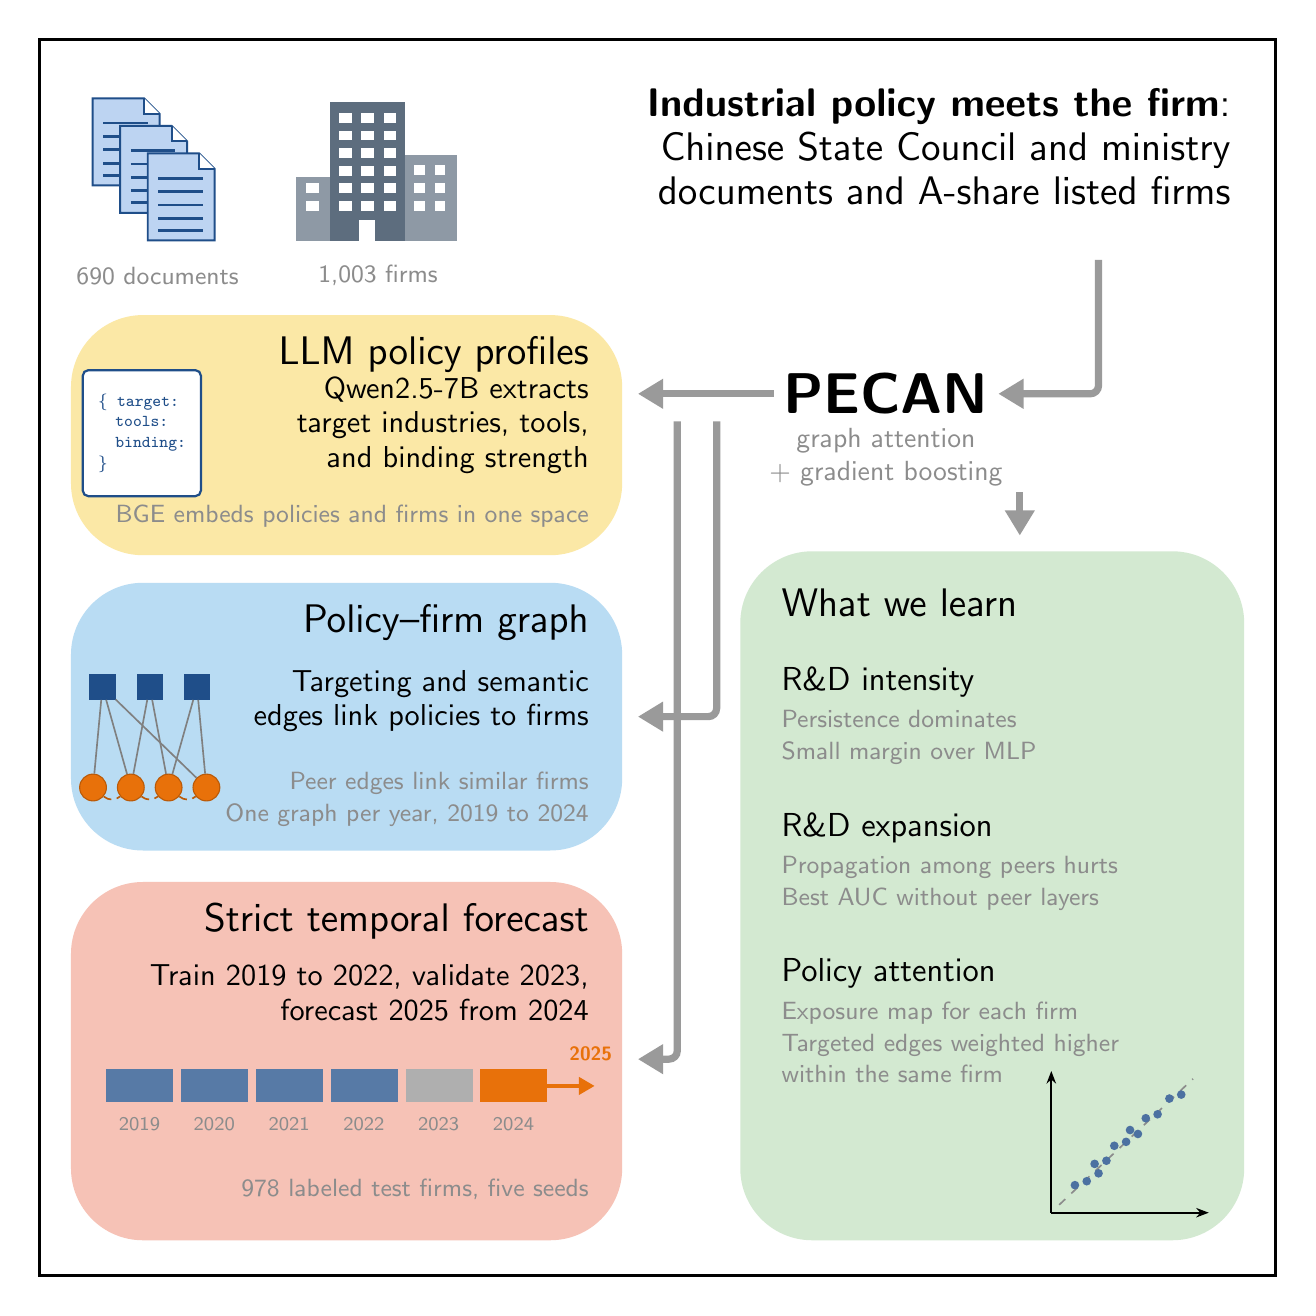
\begin{tikzpicture}[x=1cm, y=1cm]
% canvas 16 x 16 cm with a thin frame, as in Cell graphical abstracts
\fill[white] (0,0) rectangle (16,16);
\draw[line width=1.2pt] (0.15,0.15) rectangle (15.85,15.85);

% ================= top: data =================
\docicon{1.25}{14.55}{0.85}
\docicon{1.6}{14.2}{0.85}
\docicon{1.95}{13.85}{0.85}
\node[font=\fontsize{9}{10}\selectfont, text=note] at (1.65,12.85) {690 documents};
\buildingicon{4.55}{14.15}{0.95}
\node[font=\fontsize{9}{10}\selectfont, text=note] at (4.45,12.85) {1,003 firms};

\node[font=\fontsize{13.5}{16}\selectfont, anchor=north east, align=right] (data) at (15.4,15.35)
  {\textbf{Industrial policy meets the firm}:\\
   Chinese State Council and ministry\\ documents and A-share listed firms};

% ================= centre hub =================
\node[font=\fontsize{20}{22}\selectfont\bfseries, align=center] (hub) at (10.9,11.35) {PECAN};
\node[font=\fontsize{10}{12}\selectfont, text=note, align=center] at (10.9,10.55)
  {graph attention\\+ gradient boosting};
\draw[garrow] (13.6,13.05) -- (13.6,11.35) -- (hub.east);

% ================= yellow: LLM profiles =================
\fill[blobYellow, blob] (0.55,9.3) rectangle (7.55,12.35);
% JSON card icon
\begin{scope}[shift={(1.45,10.85)}]
  \draw[navy, fill=white, line width=0.8pt, rounded corners=2pt] (-0.75,-0.8) rectangle (0.75,0.8);
  \node[font=\fontsize{6.5}{7.5}\selectfont\ttfamily, text=navy, align=left] at (0,0)
    {\{ target:\\ \ \ tools:\\ \ \ binding:\\ \}};
\end{scope}
\node[head] at (7.25,11.85) {LLM policy profiles};
\node[body] at (7.25,10.95) {Qwen2.5-7B extracts\\target industries, tools,\\and binding strength};
\node[gnote] at (7.25,9.8) {BGE embeds policies and firms in one space};

% ================= blue: graph =================
\fill[blobBlue, blob] (0.55,5.55) rectangle (7.55,8.95);
\begin{scope}[shift={(1.55,6.95)}, scale=0.8]
  \foreach \i/\x in {1/-0.75,2/0,3/0.75}
    \node[draw=navy, fill=navy, minimum size=0.32cm, inner sep=0pt] (p\i) at (\x,0.85) {};
  \foreach \i/\x in {1/-0.9,2/-0.3,3/0.3,4/0.9}
    \node[circle, draw=orange!80!black, fill=orange, minimum size=0.34cm, inner sep=0pt] (f\i) at (\x,-0.75) {};
  \foreach \a/\b in {1/1,1/2,2/2,2/3,3/3,3/4,1/4}
    \draw[gray, line width=0.6pt] (p\a) -- (f\b);
  \draw[densely dashed, orange!80!black, line width=0.6pt] (f1) to[bend right=40] (f2);
  \draw[densely dashed, orange!80!black, line width=0.6pt] (f2) to[bend right=40] (f3);
  \draw[densely dashed, orange!80!black, line width=0.6pt] (f3) to[bend right=40] (f4);
\end{scope}
\node[head] at (7.25,8.45) {Policy--firm graph};
\node[body] at (7.25,7.45) {Targeting and semantic\\edges link policies to firms};
\node[gnote] at (7.25,6.2) {Peer edges link similar firms\\One graph per year, 2019 to 2024};

% ================= red: temporal forecast =================
\fill[blobRed, blob] (0.55,0.6) rectangle (7.55,5.15);
\node[head] at (7.25,4.65) {Strict temporal forecast};
\node[body] at (7.25,3.75) {Train 2019 to 2022, validate 2023,\\forecast 2025 from 2024};
% timeline icon
\begin{scope}[shift={(1.0,2.35)}]
  \foreach \k in {0,1,2,3} \fill[navy!75] ({\k*0.95},0) rectangle ++(0.85,0.42);
  \fill[note!70] (3.8,0) rectangle ++(0.85,0.42);
  \fill[orange] (4.75,0) rectangle ++(0.85,0.42);
  \foreach \k/\y in {0/2019,1/2020,2/2021,3/2022,4/2023,5/2024}
    \node[font=\fontsize{7.5}{8}\selectfont, text=note] at ({\k*0.95+0.42},-0.28) {\y};
  \draw[-{Triangle[length=2mm,width=2.2mm]}, line width=1.2pt, orange] (5.6,0.21) -- (6.2,0.21);
  \node[font=\fontsize{7.5}{8}\selectfont\bfseries, text=orange] at (6.15,0.62) {2025};
\end{scope}
\node[gnote] at (7.25,1.25) {978 labeled test firms, five seeds};

% ================= green: findings =================
\fill[blobGreen, blob] (9.05,0.6) rectangle (15.45,9.35);
\node[font=\fontsize{15}{17}\selectfont, anchor=north west] at (9.45,9.0) {What we learn};

\node[rhead] at (9.45,8.0) {R\&D intensity};
\node[rnote] at (9.45,7.45) {Persistence dominates\\Small margin over MLP};

\node[rhead] at (9.45,6.15) {R\&D expansion};
\node[rnote] at (9.45,5.6) {Propagation among peers hurts\\Best AUC without peer layers};

\node[rhead] at (9.45,4.3) {Policy attention};
\node[rnote] at (9.45,3.75) {Exposure map for each firm\\Targeted edges weighted higher\\within the same firm};

% mini scatter icon
\begin{scope}[shift={(13.0,0.95)}]
  \draw[line width=0.7pt, -{Stealth[length=1.6mm]}] (0,0) -- (2.0,0);
  \draw[line width=0.7pt, -{Stealth[length=1.6mm]}] (0,0) -- (0,1.8);
  \draw[dashed, note, line width=0.6pt] (0.1,0.1) -- (1.8,1.7);
  \foreach \x/\y in {0.3/0.35,0.45/0.4,0.55/0.62,0.7/0.66,0.8/0.85,0.95/0.9,1.1/1.0,1.2/1.2,1.35/1.25,1.5/1.45,0.6/0.5,1.0/1.05,1.65/1.5}
    \fill[navy!80] (\x,\y) circle (0.055);
\end{scope}

% ================= hub arrows =================
\draw[garrow] (hub.west) -- (7.75,11.35);
\draw[garrow] (8.75,11.0) -- (8.75,7.25) -- (7.75,7.25);
\draw[garrow] (8.25,11.0) -- (8.25,2.9) -- (7.75,2.9);
\draw[garrow] (12.6,10.1) -- (12.6,9.55);
\end{tikzpicture}
\end{document}
